\documentclass[border=4pt]{standalone}
\usepackage[T1]{fontenc}
\usepackage{helvet}
\renewcommand{\familydefault}{\sfdefault}
\usepackage{graphicx}
\usepackage{caption}
\usepackage{amsmath}
\captionsetup{font={sf,footnotesize},labelfont={sf,bf,footnotesize},justification=justified,singlelinecheck=false}
\begin{document}
\setcounter{figure}{0}
\begin{minipage}{2.68in}
\centering
\begin{figure}[htbp]
    \centering
    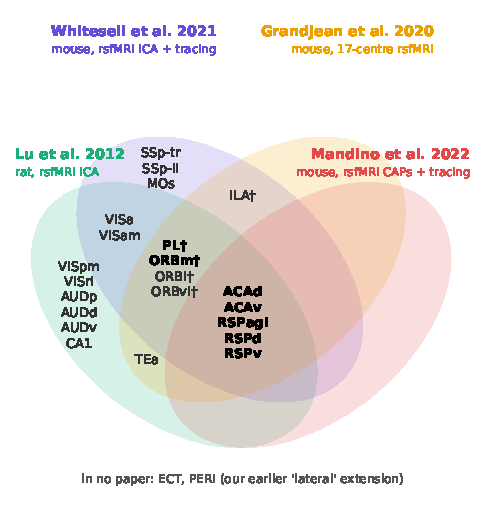
\includegraphics[width=\linewidth]{fig1_regions_panels.pdf}
    \caption{Cortical (Beryl) regions assigned to the DMN by four rodent rsfMRI studies (methods in section 1); \textdagger{} prefrontal subregions not specified by Grandjean et al., mapped here to PL, ILA and ORB. Bold: the conservative core used in this report. Subcortical DMN elements are not shown.}
    \label{fig:grey_regions}
\end{figure}
\end{minipage}
\end{document}
